\documentclass[12pt, a4paper]{article}

\usepackage{lastpage}
\usepackage{mathtools}
\usepackage{xltxtra}
\usepackage{libertine}
\usepackage{amsmath}
\usepackage{amsthm}
\usepackage{amsfonts}
\usepackage{amssymb}
\usepackage{enumitem}
\usepackage{xcolor}
\usepackage[left=1.5cm, right=1.5cm, top=2cm, bottom=2cm, bindingoffset=0cm, headheight=15pt]{geometry}
\usepackage{fancyhdr}
\usepackage[russian]{babel}
% \usepackage[utf8]{inputenc}
\usepackage{catchfilebetweentags}
\usepackage{accents}
\usepackage{calc}
\usepackage{etoolbox}
\usepackage{mathrsfs}
\usepackage{wrapfig}

\providetoggle{useproofs}
\settoggle{useproofs}{false}

\pagestyle{fancy}
\lfoot{M3137y2019}
\rhead{\thepage\ из \pageref{LastPage}}

\newcommand{\R}{\mathbb{R}}
\newcommand{\Q}{\mathbb{Q}}
\newcommand{\C}{\mathbb{C}}
\newcommand{\Z}{\mathbb{Z}}
\newcommand{\B}{\mathbb{B}}
\newcommand{\N}{\mathbb{N}}

\newcommand{\const}{\text{const}}

\newcommand{\teormin}{\textcolor{red}{!}\ }

\DeclareMathOperator*{\xor}{\oplus}
\DeclareMathOperator*{\equ}{\sim}
\DeclareMathOperator{\Ln}{\text{Ln}}
\DeclareMathOperator{\sign}{\text{sign}}
\DeclareMathOperator{\Sym}{\text{Sym}}
\DeclareMathOperator{\Asym}{\text{Asym}}
% \DeclareMathOperator{\sh}{\text{sh}}
% \DeclareMathOperator{\tg}{\text{tg}}
% \DeclareMathOperator{\arctg}{\text{arctg}}
% \DeclareMathOperator{\ch}{\text{ch}}

\DeclarePairedDelimiter{\ceil}{\lceil}{\rceil}
\DeclarePairedDelimiter{\abs}{\left\lvert}{\right\rvert}

\setmainfont{Linux Libertine}

\theoremstyle{plain}
\newtheorem{axiom}{Аксиома}
\newtheorem{lemma}{Лемма}

\theoremstyle{remark}
\newtheorem*{remark}{Примечание}
\newtheorem*{exercise}{Упражнение}
\newtheorem*{consequence}{Следствие}
\newtheorem*{example}{Пример}
\newtheorem*{observation}{Наблюдение}

\theoremstyle{definition}
\newtheorem{theorem}{Теорема}
\newtheorem*{definition}{Определение}
\newtheorem*{obozn}{Обозначение}

\setlength{\parindent}{0pt}

\newcommand{\dbltilde}[1]{\accentset{\approx}{#1}}
\newcommand{\intt}{\int\!}

% magical thing that fixes paragraphs
\makeatletter
\patchcmd{\CatchFBT@Fin@l}{\endlinechar\m@ne}{}
  {}{\typeout{Unsuccessful patch!}}
\makeatother

\newcommand{\get}[2]{
    \ExecuteMetaData[#1]{#2}
}

\newcommand{\getproof}[2]{
    \iftoggle{useproofs}{\ExecuteMetaData[#1]{#2proof}}{}
}

\newcommand{\getwithproof}[2]{
    \get{#1}{#2}
    \getproof{#1}{#2}
}

\newcommand{\import}[3]{
    \subsection{#1}
    \getwithproof{#2}{#3}
}

\newcommand{\given}[1]{
    Дано выше. (\ref{#1}, стр. \pageref{#1})
}

\renewcommand{\ker}{\text{Ker }}
\newcommand{\im}{\text{Im }}
\newcommand{\grad}{\text{grad}}

\lhead{Конспект по матанализу}
\cfoot{}
\rfoot{Лекция 5}

\begin{document}

\begin{theorem}
    %<*обобщеннаятеоремаоплотности>
    Обобщенная теорема о плотности.

    $\Phi:Segm\langle a,b\rangle\to\R$ --- аддитивная функция промежутка

    $f:\langle a,b\rangle\to\R$ --- непр.

    $\forall \Delta\in Segm\langle a,b\rangle\ \ \exists m_\Delta, M_\Delta$ --- не точный минимум/максимум

    \begin{enumerate}
        \item $m_\Delta l_\Delta\leq \Phi(\Delta)\leq M_\Delta l_\Delta$
        \item $m_\Delta\leq f(x)\leq M_\Delta$ при всех $x\in\Delta$
        \item $\forall$ фикс. $x\quad$ $M_\Delta-m_\Delta\xrightarrow[\text{``}\Delta\to x\text{''}]{} 0$
        
        $\forall \varepsilon>0 \ \ \exists \delta>0 \ \ \forall \Delta: l_\Delta<\delta \quad |M_\Delta-m_\Delta|<\varepsilon$
    \end{enumerate}

    Тогда $\forall [p,q]\in Segm\langle a,b] \quad \Phi([p,q])=\int\limits_p^q f$
    %</обобщеннаятеоремаоплотности>
\end{theorem}
%<*обобщеннаятеоремаоплотностиproof>
\begin{proof}
    $F(x)=\begin{cases}
        0, & x=a \\
        \Phi[a,x], & x>a
    \end{cases}$

    Докажем, что $F$ --- первообразная $f$.

    Фиксируем $x$

    По 1.:
    $$m_\Delta\leq\frac{F(x+h)-F(x)}{h}=\frac{\Phi[x,x+h]}{h}\leq M_\Delta$$

    По 2.:
    $$m_\Delta\leq f(x)\leq M_\Delta$$

    $$\left|\frac{F(x+h)-F(x)}{h}-f(x)\right|\leq M_\Delta-m_\Delta\xrightarrow[\text{``}\Delta\to x\text{''}]{}0$$

    Мы не можем написать ``$\Delta\to x$'' без кавычек, т.к. $\Delta$ --- не число, но ``$\Delta\to x$''$\Leftrightarrow h\to0$

    Таким образом, $$\frac{F(x+h)-F(x)}{h}-f(x)\xrightarrow[h\to0]{}0$$
\end{proof}
%</обобщеннаятеоремаоплотностиproof>

\subsection*{Объемы фигур вращения}

Объем это $V: Fig\to\R$:
\begin{enumerate}
    \item $V$ --- кон., адд.: $V(A_1\sqcup A_2)=V(A_1)+V(A_2)$
    \item $V(\text{ед. куб})=1$
    \item $V$ не меняется при движении
\end{enumerate}

Проблема: такой функции не существует.

Поэтому будем использовать объем для частных случаев фигур, а не для всех.

%<*вращениефигуры>
\begin{definition}
    $\sphericalangle A\in\R^2$ --- фигура в I квадранте.

    \textbf{Вращение} $A$:
    \begin{enumerate}
        \item по оси $x$ : $A_x=\{(x,y,z)\in\R^3 : (x,\sqrt{y^2+z^2})\in A\}$
        \item по оси $y$ : $A_y=\{(x,y,z)\in\R^3 : (\sqrt{x^2+z^2}, y)\in A\}$
    \end{enumerate}
\end{definition}

Для непр. $f:[a,b]\to\R, c\mapsto \tilde c\geq 0:$
$$\Phi(\Delta)=V(\text{ПГ}(f,\Delta)_x) \textit{(или $y$)}$$
%</вращениефигуры>

\begin{theorem}
    %<*объемвращения>
    $f:\langle a,b\rangle\to\R$ --- непр., $f\geq 0$

    $\Phi_x(\Delta)=$ ``объем фигуры вращения вокруг оси $OX$''

    $\Phi_y(\Delta)=$ ``объем фигуры вращения вокруг оси $OY$''

    Тогда : $\forall \Delta = [p,q]\in Segm\langle a,b\rangle:$
    \begin{enumerate}
        \item $\Phi_x[p,q]=\pi\int\limits_p^q f^2(x)dx$
        \item $\Phi_y[p,q]=2\pi\int\limits_p^q xf(x)dx$
    \end{enumerate}
    %</объемвращения>
\end{theorem}
%<*объемвращенияproof>
\begin{proof}
    \begin{enumerate}
        \item Это --- упражнение, оно не использует ничего умного.
        
        На лекции было сказано, что это доказывается через плотность аналогично площади криволинейного сектора.
        
        \item Мы знаем, что объем цилиндра $=S(\text{основание})\cdot h$.
        
        Для оценки $\Phi(\Delta)$ найдем прямоугольник, который является минимальным по площади сечения и максимальный прямоугольники: $\Pi_{min}$ и $\Pi_{max}$.

        \begin{figure}[h]
            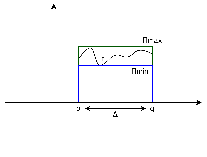
\includegraphics[scale=2.5]{images/rotation.pdf}
            \centering
        \end{figure}

        Покажем, что $2\pi x f(x)$ подходит под обобщенную теорему о плотности для $\Phi$:
        $$V((\Pi_{\min})_y)\leq \Phi(\Delta)\leq V((\Pi_{\max})_y)$$
        $$V((\Pi_{\max})_y) = S_\text{кольца} \max_{x\in[p, q]} f = \pi (q - p) (q + p) \max_{x\in[p, q]} f \le \pi (q-p) \overbrace{\max_{x\in[p, q]} 2x}^{=2q\ge q+p} \max_{x\in[p, q]} f$$
        $$V((\Pi_{\min})_y) \ge \pi \min 2x (q-p) \min f$$
        $$M_\Delta := \pi\max_{x\in[p, q]} 2x \max_{x\in[p, q]} f(x) \quad m_\Delta := \pi \min_{x\in[p, q]} 2x \min_{x\in[p, q]} f(x)$$
        \textcolor{red}{На лекции было дано $m_\Delta$ и $M_\Delta$ без $\pi$.}

        Все три условия теоремы очевидно выполнены:
        \begin{enumerate}
            \item $m_\Delta (q-p) \le \Phi(\Delta) \le M_\Delta (q-p)$
            \item $m_\Delta \le 2\pi x f(x) \le M_\Delta \quad \forall x\in \Delta$
            \item $\pi(\max f \max 2x - \min f \min 2x) \xrightarrow[\text{``}\Delta\to x\text{''}]{}0$
        \end{enumerate}
    \end{enumerate}
\end{proof}
%</объемвращенияproof>

\begin{example}
    Объем тора.

    Будем вращать окружность, центр которой лежат на оси $OX$ в точке $R$, с радиусом $r$, относительно оси $OY$.

    $$\frac{1}{2}V=2\pi \int\limits_{R-2}^{R+2}(x\mp R)\sqrt{r^2-(x-R)^2}dx=\pi\int\limits_{R_2}^{R+2} 2(x-R)\sqrt{r^2-(x-R)^2}dx+2\pi\int\limits_{R-2}^{R+2} R\sqrt{r^2-(x-r)^2}dx=$$
    $$=-\pi\frac{1}{3}(r^2-(x-R)^2)^{\frac{3}{2}}|_{x=R-2}^{x=R+2}+2\pi R\frac{\pi r^2}{2}=2\pi R\cdot \pi r^2$$
\end{example}

\subsection*{Длина гладкого пути}

%<*гладкийпуть>
$\gamma:[a,b]\to\R^m$ --- непр.

$\gamma(a)$ --- начало; $\gamma(b)$ --- конец

$\gamma:t\mapsto \begin{pmatrix}
    \gamma_1(t) \\
    \gamma_2(t) \\
    \vdots \\
    \gamma_m(t)
\end{pmatrix}$; $\gamma_i$ --- коорд. функции

Если все $\gamma_i\in C^1 [a,b]$, то $\gamma$ --- \textbf{гладкий путь}.

$C_\gamma := \gamma([a, b])$ --- \textbf{носитель пути}.
%</гладкийпуть>

%<*векторскорости>

Вектор скорости:
$$\gamma'(t)=\lim\limits_{\Delta t\to0}\frac{\gamma(t+\Delta t)-\gamma(t)}{\Delta t}=\lim \begin{pmatrix}
    \frac{\gamma_1(t+\Delta t)-\gamma_1(t)}{\Delta t} \\
    \vdots \\
    \frac{\gamma_m(t+\Delta t)-\gamma_m(t)}{\Delta t} \\
\end{pmatrix}=\begin{pmatrix}
    \gamma_1'(t) \\
    \gamma_2'(t) \\
    \vdots \\
    \gamma_m'(t)
\end{pmatrix}$$
%</векторскорости>

Кривая Пеано: $[0,1]\to[0,1]\times[0,1]$ --- ломает длину пути, но она не гладкая, поэтому мы рассматриваем только гладкие пути.

\begin{definition}
    %<*длинагладкогопути>
    \textbf{Длина пути} --- фукнция $l$, заданная на множестве гладких путей в $\R^m$, такая что:
    \begin{enumerate}
        \item $l\geq 0$
        \item $l$ --- аддитивна: $\forall [a,b] \ \ \forall \gamma:[a,b]\to\R^m \ \ \forall c\in(a,b) \quad l(\gamma)=l(\gamma|_{[a,c]})+l(\gamma|_{[c,b]})$
        \item $\forall \gamma, \tilde \gamma$ --- гладкие пути, $C_\gamma, C_{\tilde \gamma}$ --- носители путей
        
        Если $\exists T : C_\gamma\to C_{\tilde\gamma}$ --- сжатие: $(\forall M, M' \ \ \rho(T(M), T(M'))\leq \rho(M, M'))$, тогда $l(\tilde\gamma)\leq l(\gamma)$

        \item Нормировка: $\gamma$ --- гладкий путь, $\gamma(t)=vt+u; \ \ u,v\in\R^m$:
        $$l(\gamma)=\rho(\gamma(a), \gamma(b))$$
    \end{enumerate}
    %</длинагладкогопути>
\end{definition}

Свойства:
\begin{enumerate}
    \item ``Длина пути'' $\geq$ ``длина хорды''
    \item При растяжениях длина растет.
    \item Длина не меняется при движении.
\end{enumerate}

% Существование длины пути:

\begin{definition}
    %<*вариацияфункции>
    $\gamma: [a,b]\to\R^n \quad t_0=a<t_1<t_2<\ldots<t_n=b$

    $\tau=\{t_0\ldots t_n\}$ --- дробление отрезка.

    Тогда \textbf{вариация функции} $\gamma$ на отрезке $[a, b]$ это $l$:
    $$l(\gamma)=\sup_\tau\Big\{\sum\limits_{i=1}^n \rho(\gamma(t_{i-1}), \gamma(t_i))\Big\}$$
    %</вариацияфункции>
\end{definition}

\begin{lemma}
    Вариация $\gamma$ на отрезке $[a, b]$ --- длина пути $\gamma$.
\end{lemma}
\begin{proof}
    Тривиальная проверка определения длины пути. \textcolor{red}{Кохась не говорил, но надо доказать.}
\end{proof}

\begin{example}
    Рассмотрим путь из $A$ в $B$, который проходится за $1$ час со скоростью $5$ км/ч. Длина этого пути --- $5$ км.
\end{example}

\begin{theorem}
    %<*длинапутивrm>
    $\gamma\in C^1([a,b]\to\R^m)$

    Тогда $l(\gamma)=\int\limits_a^b ||\gamma'(t)||dt$
    %</длинапутивrm>
\end{theorem}
%<*длинапутивrmproof>
\begin{proof}
    Будем считать $\gamma'\not=0$, $\gamma$ --- инъективная.

    $\Phi: [p,q]\subset [a,b]\mapsto l(\gamma|_{[p,q]})$ --- адд. ф-ция промежутка.

    Докажем, что $f(t)=||\gamma'(t)||$ --- плотность $\Phi$

    $$\Delta\subset [a,b] \quad m_i(\Delta):=\min\limits_{t\in\Delta}|\gamma'_i(t)| \quad M_i(\Delta)=\max|\gamma'_i(t)|$$
    $$m_\Delta=\sqrt{\sum\limits_{i=1}^m m_i(\Delta)^2} \quad M_\Delta=\sqrt{\sum\limits_{i=1}^m M_i(\Delta)^2}$$
    Докажем, что $m_\Delta l_\Delta\leq \Phi(\Delta)\leq M_\Delta l_\Delta$

    $\tilde \gamma : \Delta\to\R^m$ --- лин. путь

    $\tilde \gamma(t)=\vec M\cdot t$, где $\vec M=\begin{pmatrix}
        M_1(\Delta) & \ldots & M_m(\Delta)
    \end{pmatrix}$

    $T: C_{\gamma|_\Delta}\to C_{\tilde \gamma} \quad \gamma(t)\mapsto \tilde \gamma(t)$

    Утверждение: $T$ --- растяжение.
    $$||\vec Mq - \vec Mp||=(q-p)||\vec M||=(q-p)M_\Delta$$

    $$\rho(\gamma(t_0), \gamma(t_1))=\sqrt{\sum\limits_{i=1}^m (\gamma_i(t_0)-\gamma_i(t_1))^2}\stackrel{\text{т. Лагранжа}}{=}\sqrt{\sum\limits_{i=1}^m \gamma_i'(\overline t_i)^2 (t_0-t_1)^2}\leq ||\vec M||\cdot|t_0-t_1|=$$
    $$=\rho(\tilde\gamma(t_0), \tilde\gamma(t_1))=\rho(T(\gamma(t_0)), T(\gamma(t_1)))$$
\end{proof}
%</длинапутивrmproof>

%<*длинапутивrmaltproof>
\begin{proof}
    \textit{(альтернативное)}.
    
    Покажем, что $\int ||\gamma'||$ удовлетворяет всем требованиям длины гладкого пути:
    \begin{enumerate}
        \item $\forall \gamma \ \ l(\gamma)\ge 0$ --- очевидно, т.к. $||\gamma'||\ge 0$
        \item Линейность: очевидно по линейности определенного интеграла.
        \item Сжатие: $\exists T : C_\gamma \to C_{\tilde \gamma}$
        $$\gamma'(t) = \lim_{h\to0} \frac{\gamma(t + h) - \gamma(t)}{h}$$
        $$||\gamma'(t)||=\lim_{h\to0} \frac{||\gamma(t + h), \gamma(t)||}{|h|}$$
        $$||\gamma'(t)||=\lim_{h\to0} \frac{\rho(\gamma(t + h), \gamma(t))}{|h|} \quad ||\tilde \gamma'(t)||=\lim_{h\to0} \frac{\rho(\tilde \gamma(t + h), \tilde \gamma(t))}{|h|}$$
        $$\rho(\gamma(t + h), \gamma(t)) \ge \rho(\tilde \gamma(t + h), \tilde \gamma(t)) \Rightarrow ||\gamma'(t)|| \ge ||\tilde \gamma'(t)|| \Rightarrow l(\gamma)\ge l(\tilde \gamma)$$
        \item Нормировка. $\sphericalangle \gamma : \gamma(t) = \vec u + \vec v t$
        $$l(\gamma) = \int_a^b ||\vec v|| dt = ||\vec v|| (b-a)$$
        $$\rho(\gamma(a), \gamma(b)) = ||\vec u + \vec v a - \vec u - \vec v b|| = ||\vec v(a-b)|| = \sqrt{\sum_{i=1}^m v_i^2 (b-a)^2}=(b-a)||\vec v||$$
    \end{enumerate}
\end{proof}
%</длинапутивrmaltproof>

\begin{example}
    %<*длинаграфика>
    Длина графика $y = f(x), f\in C^1$ на отрезке $[a, b]$

    $$\gamma(x)=\begin{pmatrix}
        x \\
        f(x)
    \end{pmatrix} \quad \gamma'(x) = \begin{pmatrix}
        1 \\
        f'(x)
    \end{pmatrix} \quad ||\gamma'(x)|| = \sqrt{1+(f'(x))^2}$$
    $$l = \int_a^b \sqrt{1+(f'(x))^2}dx$$
    %</длинаграфика>
\end{example}

\begin{example}
    %<*длинавполярных>
    Длина кривой $r=r(\varphi)$ в полярных координатах, $\varphi\in[\alpha, \beta]$
    $$x=r(\varphi)\cos\varphi \quad y=r(\varphi)\sin\varphi$$
    $$\gamma'(\varphi)=\begin{pmatrix}
        r'(\varphi)\cos\varphi - r(\varphi)\sin\varphi \\
        r'(\varphi)\sin\varphi + r(\varphi)\cos\varphi
    \end{pmatrix}$$
    $$||\gamma'(\varphi)||=\sqrt{(r'(\varphi))^2+(r(\varphi))^2-2r'(\varphi)r(\varphi)\cos\varphi\sin\varphi+2r'(\varphi)r(\varphi)\cos\varphi\sin\varphi}$$
    $$||\gamma'(\varphi)||=\sqrt{(r'(\varphi))^2+(r(\varphi))^2}$$
    $$l=\int_\alpha^\beta\sqrt{r^2+(r')^2}d\varphi$$
    %</длинавполярных>
\end{example}

\end{document}